\documentclass[10pt,conference,compsocconf]{IEEEtran}

%\usepackage{times}
%\usepackage{balance}
\usepackage{url}
\usepackage{graphicx}	% For figure environment
\usepackage{color}
\usepackage{subcaption}
\usepackage{hyperref}
\usepackage{gensymb}

\newcommand{\todo}[1]{{\color{red}{\textbf{TODO: #1}}}}
\newcommand{\conv}[3]{$ \cal{C} $(#1$ \times  $#1, #2, #3)}
\newcommand{\relu}{$ \cal{R}~$}
\newcommand{\maxpool}[2]{$ \cal{M} $(#1$ \times $#1, #2)}
\newcommand{\lrn}{$ \cal{LRN}~$}
\newcommand{\fc}[2]{$ \cal{FC} $(#1, #2)}

\begin{document}
\title{Road Extraction from Aerial Images}
\author{
  Delio Vicini, Matej Hamas, Taivo Pungas\\
  Department of Computer Science, ETH Zurich, Switzerland
}

\maketitle

\begin{abstract}
In this paper, we present a novel method to automatically segment aerial images in road and non-road patches. Our technique classifies small image patches using a deep convolutional neural network. On top of the neural network, we apply a post-processing filter based on a support vector machine classifier. The combination of convolutional neural network and post-processing yields a prediction accuracy over 90\% on a representative benchmark data set.
\end{abstract}

\section{Introduction}
\label{sec:intro}

In this paper, we present a novel technique for detecting roads on aerial images. The solution to this problem has potentially many application ranging from automation of map making to urban planning and environmental monitoring.

Given an RGB aerial or satellite image of a moderate resolution, we seek to classify each 16x16 patch as \textit{road} or \textit{non-road}. Hence, this is an instance of a binary classification problem (Figure \ref{sec:intro}).

As this is quite long-standing problem in computer vision, and thanks to its many applications, there is rich previous work in this area \cite{Huang.2002} \cite{MnihThesis.2013} \cite{Long.2014} \cite{Montoya.2015} \cite{Saito.2015}. Most of the past work concentrated on per-pixel prediction from aerial images. Some papers also look at multi-class semantic classification by introducing specific \textit{building} class \cite{Saito.2015}. 

Previous approaches include support vector machines (SVMs) on manually extracted features \cite{Huang.2002}, convolutional neural networks (CNNs) \cite{Long.2014} \cite{Saito.2015}, conditional random fields \cite{Montoya.2015} and other probabilistic approaches.

Unlike most of the previous work, we concentrate on per-patch and not on per-pixel prediction. We have developed a novel solution by combining a deep CNN with an SVM based post-processing.

We compare our approach to two different baseline algorithms. One of them is a plain vanilla 2-layer CNN with SGD optimizer. The second is the same CNN followed by a denoising step by means of dictionary filtering.

In conclusion, our main contributions are patch-based, \mbox{4-layer} CNN architecture for road segmentation followed by the SVM based post-processing scheme. 

\begin{figure}[]
	\label{fig:intro_example}
	\centering
	\begin{subfigure}{.2\textwidth}
		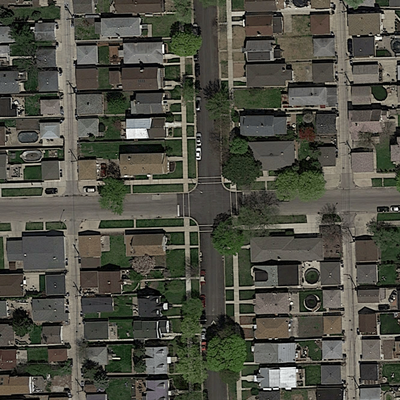
\includegraphics[width=1\textwidth]{figs/img1.png}
	\end{subfigure}
	\begin{subfigure}{.2\textwidth}
		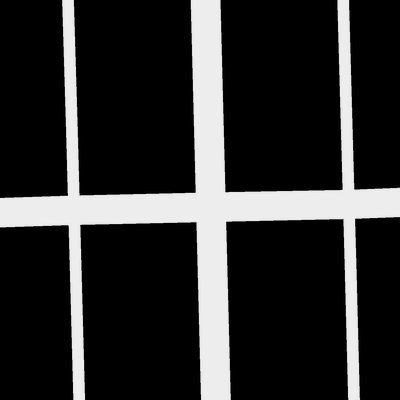
\includegraphics[width=1\textwidth]{figs/groundtruth1.png}
	\end{subfigure}
	\caption{Aerial image of an urban scene and the ground truth binary classification displaying the roads.}
\end{figure}

\section{Models and Methods}
\label{sec:MM}
In this section we describe data augmentation techniques, baseline and final CNN architectures and post-processing techniques applied on the top of the CNN output.

\subsection{Data Augmentation}
\label{subsec:preprocessing}
The lack of training data is a universal problem in machine learning. We extract patches of a particular size from input images. To enlarge the dataset, we generate more training patches by flips and rotations (\todo{Taivo, what transformations are we finally using?}). 

Afterwards, we zero-mean the training dataset by subtracting the mean image from all patches. We do not divide by standard deviation as the images are naturally well distributed.

We then generate the corresponding ground truth patches from the input images. Each ground truth patch is converted to a label 1 if the number of road pixels exceeds a threshold 0.25. It is 0 otherwise. The labels are stored in a 1-hot format, i.e. as tuples [0, 1] or [1, 0].

Finally, we balance the training dataset to include the same number of positive and negative examples. This is done to prevent the CNN from learning a bias towards one label.

\subsection{Notation - CNN Architecture}
Here, we provide a short overview of CNN layer types that are used in the following sections.
\begin{itemize}
	\item \conv{N}{I}{F} \\
	Convolutional layer with filters of size N$ \times $N, I input channels and F number of filters which corresponds to the number of output channels. The default stride is 1 both vertically and horizontally and the image is padded so it retains the size. \todo{How is image padded? I've been searching for this in tensorflow doc and code but cannot find it :(.}
	\item \maxpool{N}{S} - Max-pooling layer of size N$ \times $N, stride S.
	\item \lrn - Local response normalization layer across the current batch of training data \cite{tensorflow.2015}.
	\item \fc{I}{O} - Fully connected layer from I input channels to O output channels.
\end{itemize}

\subsection{Baseline CNN Architecture}
\label{subsec:baselineCNN}
The baseline CNN operates on patches of size $16 \times 16$. It has two convolutional and two fully connected layers with the following architecture:
\begin{center}
	\conv{5}{3}{32} -- \conv{5}{32}{64} -- \\ 
	\fc{1024}{512} -- ReLU -- \fc{512}{2}.
\end{center}
ReLU and \maxpool{2}{2} is applied after every convolutional layer.

The activation functions in the FC layers are identities. We apply \textit{softmax} to two outputs to get the probabilities for both classes. All the weights are initialized normally with standard deviation 0.1. The weights in the FC layers are L2 regularized with a factor $ 5 \times 10^{-4} $. We use a plain vanilla stochastic gradient descent (SGD) optimizer with an exponentially decaying learning rate, starting at 0.01 with a decay rate 0.95. Batch size is 16. 

\subsection{Improved CNN Architecture}
\label{subsec:CNN}
We modified the baseline CNN in various ways to improve its performance. We made it deeper, experimented with the widths of layers and filter sizes, tried using dropout or local response normalization instead of L2 regularization of FC weights, tested different optimizers (momentum and Adam) and learning rates. We also implemented cross-validation to estimate the training time after which the out-of-sample error converges.

\begin{figure}
	\centering
	\begin{subfigure}[t]{.15\textwidth}
		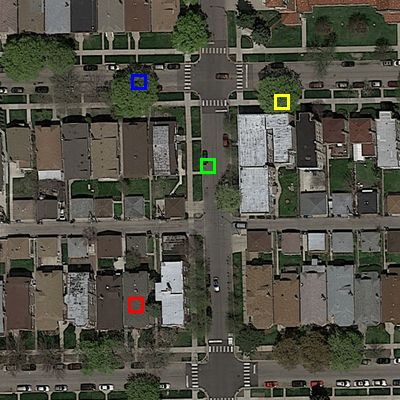
\includegraphics[width=1\textwidth]{figs/context_size/full_img}
		\caption{Input image}
	\end{subfigure}
	\begin{subfigure}[t]{.15\textwidth}
		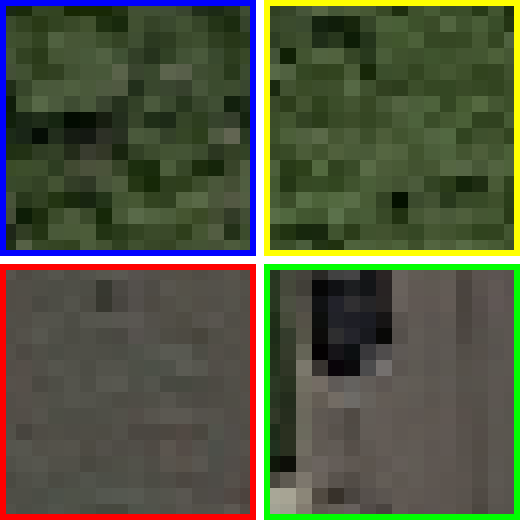
\includegraphics[width=1\textwidth]{figs/context_size/context16}
		\caption{$ 16 \times 16 $ patches}
	\end{subfigure}
	\begin{subfigure}[t]{.15\textwidth}
		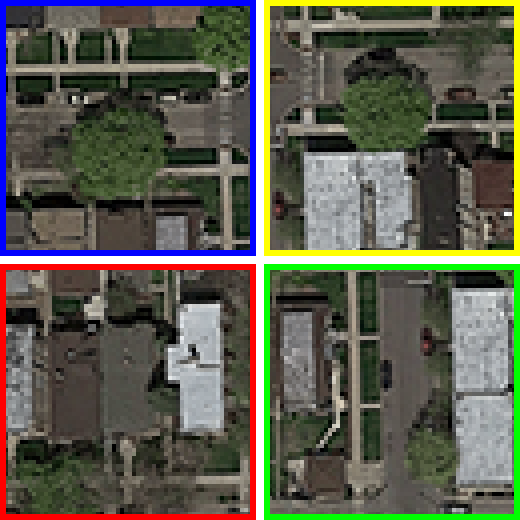
\includegraphics[width=1\textwidth]{figs/context_size/context64_ds}
		\caption{$ 64 \times 64 $ patches (extracted from the downsampled image)}
	\end{subfigure}
	\caption{Aerial image of an urban scene and some example patches. Note, that in the $ 16 \times 16 $ patches it is can be impossible to infer the correct labeling due to the limited perception of the surroundings.}
	\label{fig:context_size}
\end{figure}

Moreover, we increased the context size to $ 64\times64 $, i.e. the network predicts a label for the central $ 16\times16 $ patch using larger context. Image boundaries are handled using a mirror boundary conditions. Additionally, we downsample training and testing images by a factor of two. This means that the context considered by the neural network effectively doubles. Figure \ref{fig:context_size} shows a comparison between the context size of the baseline CNN and the context size of the improved CNN.



The final architecture of the 4-layer CNN is the following:
\begin{center}
	\conv{5}{3}{16} -- \conv{3}{16}{32} -- \\ 
	\conv{3}{32}{32} -- \conv{3}{32}{64} -- \\
	\fc{1024}{64} -- ReLU -- \fc{64}{2}.
\end{center}
After every convolutional layer, we apply ReLU, \lrn and \maxpool{2}{2}.

The activation functions in the first FC layer are identities and in the second sigmoids. We use neither dropout, nor L2 regularization of the FC weights as the local response normalization already sufficiently avoids overfitting. The class probabilities are again obtained using \textit{softmax}.

After discovering that exponential decaying learning rate does not help, we have fixed it to the empirically determined value 0.01. 
In the final model, we use the Adam optimizer algorithm \cite{Adam.2014} with $ \epsilon = 0.1 $ and the batch size is 32. All the weights are initialized normally using standard deviation 0.1.


\subsection{Post-Processing}
The convolutional neural networks output independent predictions for all $ 16 \times 16 $ patches of the processed image. The spatial arrangement of predictions however contains valuable information, which can be used to further improve the prediction accuracy. For example, it is highly unlikely to observe a road which only covers one patch. If the CNN predicts an isolated patch as belonging to the road label, we can discard this prediction with high certainty. The opposite also holds: a patch labeled as non-road surrounded by patches labeled as road is most likely part of the road as well. Oftentimes false negatives are caused by shadows or overlapping structures such as railway bridges.

\par 
The simplest post-processing scheme is therefore to simply reject outliers based on neighboring predictions. If all neighbors of a patch are assigned the label road, we can also assign the label road to the current patch. A simple scheme like this can already significantly improve prediction accuracy, because many prediction errors are isolated patches. However, more sophisticated algorithms promise even more gain in quality, as the post-processing algorithm should account for more than just the closest neighbors.

\par 
One more advanced way of reducing the noise in the CNN output is to use dictionary based denoising \cite{Elad.2006}. We do this by learning a dictionary of 100 atoms, each representing a  $ 5 \times 5 $ square of patch predictions. The dictionary is learned from the patch labels in the training data using the algorithm presented by Mairal et al. \cite{Mairal.2009}. Given the trained dictionary, we can then denoise the predictions for a test image by solving an orthogonal matching pursuit problem for each $ 5 \times 5 $ patch of patch predictions. This is done in a sliding window fashion, similar to the work by Elad et al. \cite{Elad.2006}. We found this to work quite well if the level of noise in the CNN predictions is high, which is the case in the baseline CNN. However, as the quality of the CNN improves, dictionary based denoising seems to become less useful.

\par 
In our pipeline, we filter the CNN output by predicting the label of a patch from the labels of the surrounding patches using a binary support vector machine (SVM) classifier. Given a window of $ 7 \times 7 $ patches predicted by the CNN, we predict the label of the central patch using a SVM classifier. We directly use the per-patch probabilities produced by the CNN as features for the SVM classifier. We also tried to automatically extract features using Restricted Boltzmann Machines \cite{smolensky.1986}, but could not achieve an increase in prediction accuracy.
\par
The SVM uses a radial basis function kernel and a soft-margin penalization weight of $ 1 $. We did not perform a systematic search for optimal SVM hyper-parameters, as these parameters seem to work reasonable well.
\par 
We found it beneficial to iteratively apply this denoising technique. This seems to help to propagate confident predictions, as suggested by Mnih and Geoffrey \cite{Mnih.2010}. In practice, we use only two iterations. After two iterations most noise is already removed. Increasing the number of iterations biases the predictions too much and does not lead to a gain in accuracy.

\par
We also tried using graph cut based inference \cite{Boykov.2001}. For this we computed per-pixel labels by accumulating CNN per-patch votes using a sliding window. This however did not work well, since graph cut based image segmentation relies on strong edges between fore- and background. In our aerial images, this is not the case and the boundary between road and non-road is fairly weak in terms of local edge contrast. Furthermore, the probabilities produced by the CNN are often close to 0 or 1. Graph cut based segmentation is simply not robust enough towards a locally strongly biased data term.

\par 
We also experimented using an additional CNN for post-processing, as suggested by Mnih and Geoffrey \cite{Mnih.2010}. We used a network with two convolutional and two fully connected layers, predicting the central patch from a $ 9 \times 9 $ square of patch predictions from the first CNN. However, we did not get an improvement in accuracy over the simple SVM based post-processing scheme.

\section{Results}
\label{sec:results}
The neural networks were implemented using TensorFlow \cite{tensorflow.2015} and the post processing using scikit-learn \cite{sklearn.2011}. For the baseline CNN, we used the code provided in the lecture materials, without any modifications. We trained it for around 30 minutes, which was sufficient to achieve convergence. The training was done on a cluster node with 16 cores (Intel Xeon E5-2697 v2 or Xeon E5-2680 v3 depending on availability on the Euler cluster) and 128GB of memory. Our improved CNN model trains for around 20 hours on the same hardware. The post processing SVM trains for around 1.5 hours on a conventional desktop computer (Intel Core2 Quad q9550, 4GB of memory). All neural network code runs exclusively on the CPU, since the used cluster does not provide any GPU nodes. Given the trained models, individual satellite images are processed in a matter of seconds.

\par 
We compare our method to the two different baseline implementations described previously. The first is the CNN described in Section \ref{subsec:baselineCNN}. The second one is the same CNN combined with dictionary based denoising. We measure model accuracy as the reported score in the public Kaggle leader board. Ideally, one would compute an average cross validation error, to also have an estimate of the variance of the measured accuracy. However, since CNNs are very expensive to train we decided to report the Kaggle score only.

\par
The baseline CNN achieves an accuracy of only 77.65\%. Post-processing the output from this network using learned dictionaries improves the accuracy to \todo{percent} \%. 

\par
Our improved CNN on its own achieves an accuracy of  \todo{percent}. Applying our SVM based post-processing procedure on top of these outputs, we get an accuracy of around  \todo{percent}.

\section{Discussion}
\label{sec:discussion}
The baseline CNN clearly suffers from the fact that its context size is too small. Given a $ 16 \times 16 $ image patch at the resolutions we worked with, it is oftentimes impossible to correctly decide whether this patch belongs to a road or not. Even as humans we have a hard time to take this decision. A typical example where a network with such a small context size fails are trees. In our training data, there are many cases where trees cover a road and are thus labelled as road. However, trees which stand on an open field are not part of a road. Also flat roofs can sometimes resemble roads. \todo{SHOW IMAGES WHICH ARE HARD TO CLASSIFY. SHOW FAILURES}

\par 
Adding dictionary based denoising on top of this baseline CNN improves the predictions. The dictionary based method manages well with isolated outliers. However, the prediction quality is inherently limited by the output of the underlying CNN. In contrast to image denoising, the noise produced by the CNN does not have zero-mean. Oftentimes the CNN will mispredict a whole group of patches. The dictionary based denoising then fails to infer the correct labels. 

\par 
The accuracy gain we achieve using our improved CNN is mostly due to the increased patch size. The larger context reveals much more information about the currently processed image patch. Despite the improved architecture, there are still a lot of mispredictions. 


\par
Our post-processing algorithm manages to further reduce error. In \todo{BEFORE AND AFTER FIGURE} we can see, that almost all noise has been removed. There are still some areas where the post-processing is not very successful. Sometimes, the output predicted by the CNN contains roads which do not well connect to each other. The post-processor often does not succeed in connecting these road segments. Also it seems to have a strong bias for orthogonal roads, since the test set is dominated by these road directions. We experimented with rotating the training images by $ 45\degree $, but did not succeed in improving the prediction accuracy. Our current algorithm often predicts diagonal roads to thin or even removes them partially. This is the most prominent limitation of our current approach.

\begin{figure}
	\centering
	\begin{subfigure}[t]{.2\textwidth}
		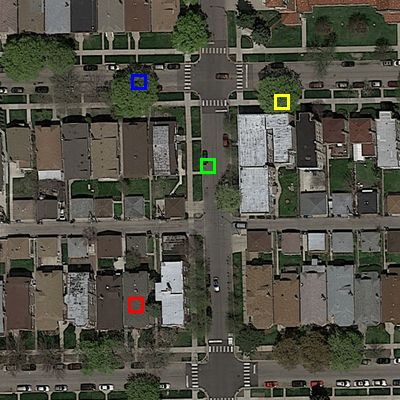
\includegraphics[width=1\textwidth]{figs/context_size/full_img}
		\caption{Raw CNN predictions}
	\end{subfigure}
	\begin{subfigure}[t]{.2\textwidth}
		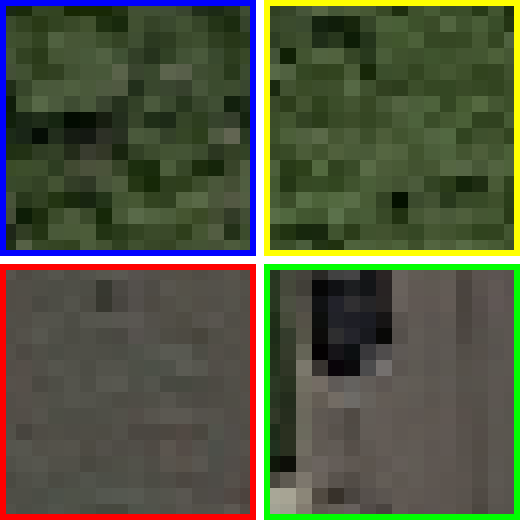
\includegraphics[width=1\textwidth]{figs/context_size/context16}
		\caption{Post-processed predictions}
	\end{subfigure}
	\caption{Results of our method and the two baseline algorithms.}
	\label{fig:post_processing}
\end{figure}

\begin{figure*}	
	\centering
	\begin{subfigure}[t]{.2\textwidth}
		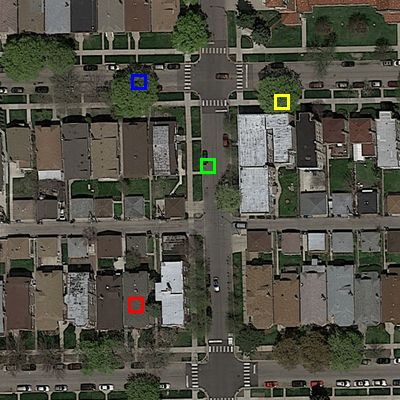
\includegraphics[width=1\textwidth]{figs/context_size/full_img}
		\caption{Input image}
	\end{subfigure}
	\begin{subfigure}[t]{.2\textwidth}
		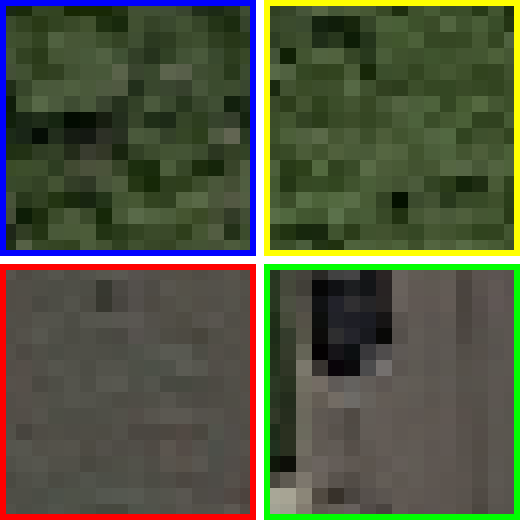
\includegraphics[width=1\textwidth]{figs/context_size/context16}
		\caption{Baseline CNN predictions}
	\end{subfigure}	
	\begin{subfigure}[t]{.2\textwidth}
		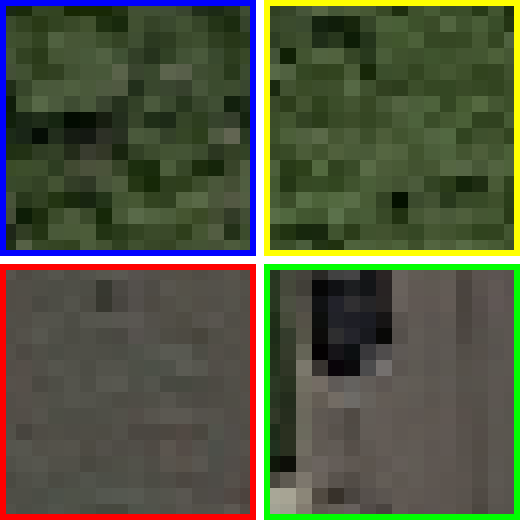
\includegraphics[width=1\textwidth]{figs/context_size/context16}
		\caption{Denoised baseline CNN predictions}
	\end{subfigure}	
	\begin{subfigure}[t]{.2\textwidth}
		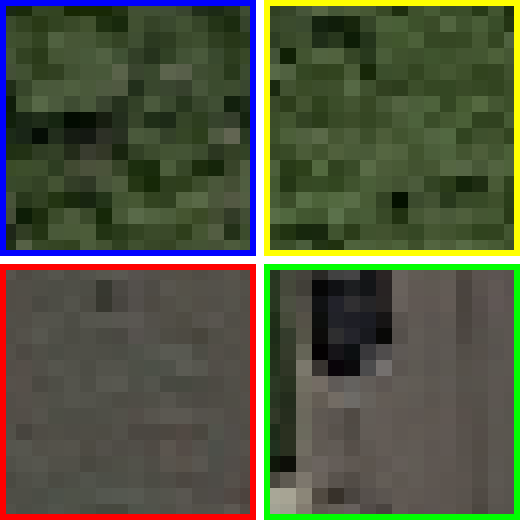
\includegraphics[width=1\textwidth]{figs/context_size/context16}
		\caption{Our predictions}
	\end{subfigure}		
	\caption{Results of the two baseline algorithms and our method.}	
	\label{fig:resuls}
\end{figure*}
\section{Summary}
\label{sec:summary}
TODO - last

\bibliographystyle{IEEEtran}
\bibliography{references}
\end{document}
